\subsection{Exercises}

%%%%%%%%%%%%%%%%%%%%%%%%%%%%%%
\Large{Problem 1.1}
\begin{figure}[H]
    \centering
    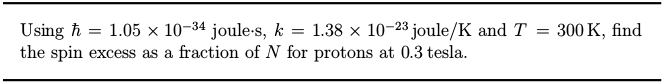
\includegraphics[width=0.8\textwidth,keepaspectratio]{prbl11}
    \label{fig:prbl11}
\end{figure}

\textit{Remember:}
\begin{itemize}
	\item This problem shows how to calculate the excess amount of spins occupying a lower energy level relative to the higher energy level, in a sample immersed in a static magnetic field.
\end{itemize}

\lstinputlisting{../project/functions/ch1/excessSpins.m}

\clearpage

\Large{Problem 1.2}
\begin{figure}[H]
    \centering
    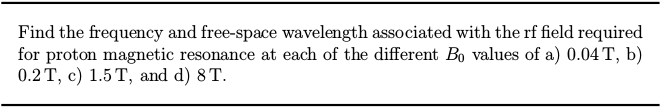
\includegraphics[width=0.8\textwidth,keepaspectratio]{prbl12}
    \label{fig:prbl12}
\end{figure}

\textit{Remember:}
\begin{itemize}
	\item This problem computes the resonance frequency of the oscillating magnetic field for a given static polarising magnetic field.
\end{itemize}

\lstinputlisting{../project/functions/ch1/resonanceFrequency.m}

\textit{Remember: (For the opposite problem)}
\begin{itemize}
	\item This problem computes the field strength associated with the frequency of an RF field for a given gyromagnetic ratio.
\end{itemize}

\lstinputlisting{../project/functions/ch1/fieldStrength.m}

